%%%%%%%% AIWILD 2026 WORKSHOP SUBMISSION %%%%%%%%%%%%%%%%%

\documentclass{article}

\usepackage{microtype}
\usepackage{graphicx}
\usepackage{subcaption}
\usepackage{booktabs}
\usepackage{hyperref}
\newcommand{\theHalgorithm}{\arabic{algorithm}}
\usepackage{../../icml2026/icml2026}
\usepackage{amsmath}
\usepackage{amssymb}
\usepackage{mathtools}
\usepackage[capitalize,noabbrev]{cleveref}

\icmltitlerunning{\raisebox{-1.5pt}{\fontsize{7}{7}\selectfont PatchSteg Agent Security}}

\begin{document}

\twocolumn[
  \icmltitle{PatchSteg: Image-Mediated Covert Channels Between Multimodal Agents}

  \begin{icmlauthorlist}
    \icmlauthor{Anonymous Authors}{anon}
  \end{icmlauthorlist}

  \icmlaffiliation{anon}{Anonymous Institution}
  \icmlcorrespondingauthor{Anonymous Author}{anonymous@example.com}
  \icmlkeywords{multimodal agents, agent security, covert channels, monitoring, latent representations}

  \vskip 0.3in
]

\printAffiliationsAndNotice{}

\begin{abstract}
Multimodal agents increasingly coordinate through shared images: screenshots, generated plans, visual tool outputs, and workspace artifacts. We show that this communication substrate can support a covert channel that is invisible to ordinary pixel inspection but recoverable by another model-aware agent. PatchSteg is a training-free post-hoc channel in which a sender perturbs selected spatial positions in a diffusion VAE latent, decodes the result to an image, and a receiver re-encodes the image to recover the signed perturbations. Across 300 CIFAR-10 images and multiple Stable Diffusion VAE backbones, stability-selected carriers recover bits reliably while revealing a reliability--stealth tradeoff under detector sweeps. We frame PatchSteg as a multi-agent security finding: monitoring agent communication requires threat models and defenses that account for representation-level channels, not only visible content.
\end{abstract}

\section{Introduction}

Agents in the wild do not communicate only through explicit text messages. They exchange images through browsers, shared workspaces, generated visualizations, screenshots, and perception pipelines. A monitor may inspect the visible image and the accompanying caption, but the agents that produce and consume the image may also share preprocessing models, latent representations, or hidden conventions.

This paper studies a concrete multi-agent security risk: image-mediated covert communication through VAE latents. A sender with access to a compatible diffusion VAE can perturb selected latent positions before decoding an image. A receiver that shares the VAE checkpoint and seed can re-encode the image and recover the message from the sign of those perturbations. The image need not contain visible symbols, text, or pixel-bit flips. The payload lives in a model-readable representation channel.

PatchSteg is our minimal demonstration of this channel. It is training-free, post-hoc, and works on existing images rather than requiring generation-time control. We use it to quantify when image-mediated communication is reliable, when detectors catch it, and what assumptions a defender needs. The result connects directly to secret-collusion findings in language agents \citep{motwani2024secret}: if text can carry covert conventions, then shared images can carry covert latent state.

Our contributions are:
\begin{enumerate}
    \item We define a threat model for image-mediated covert communication between multimodal agents through shared VAE representations.
    \item We introduce PatchSteg, a reproducible latent channel that transmits bits through decoded images and recovers them after re-encoding.
    \item We evaluate reliability, content dependence, VAE generality, robustness, and detector behavior, showing that pixel-only monitoring is an incomplete defense.
\end{enumerate}

\begin{figure*}[t]
\centering
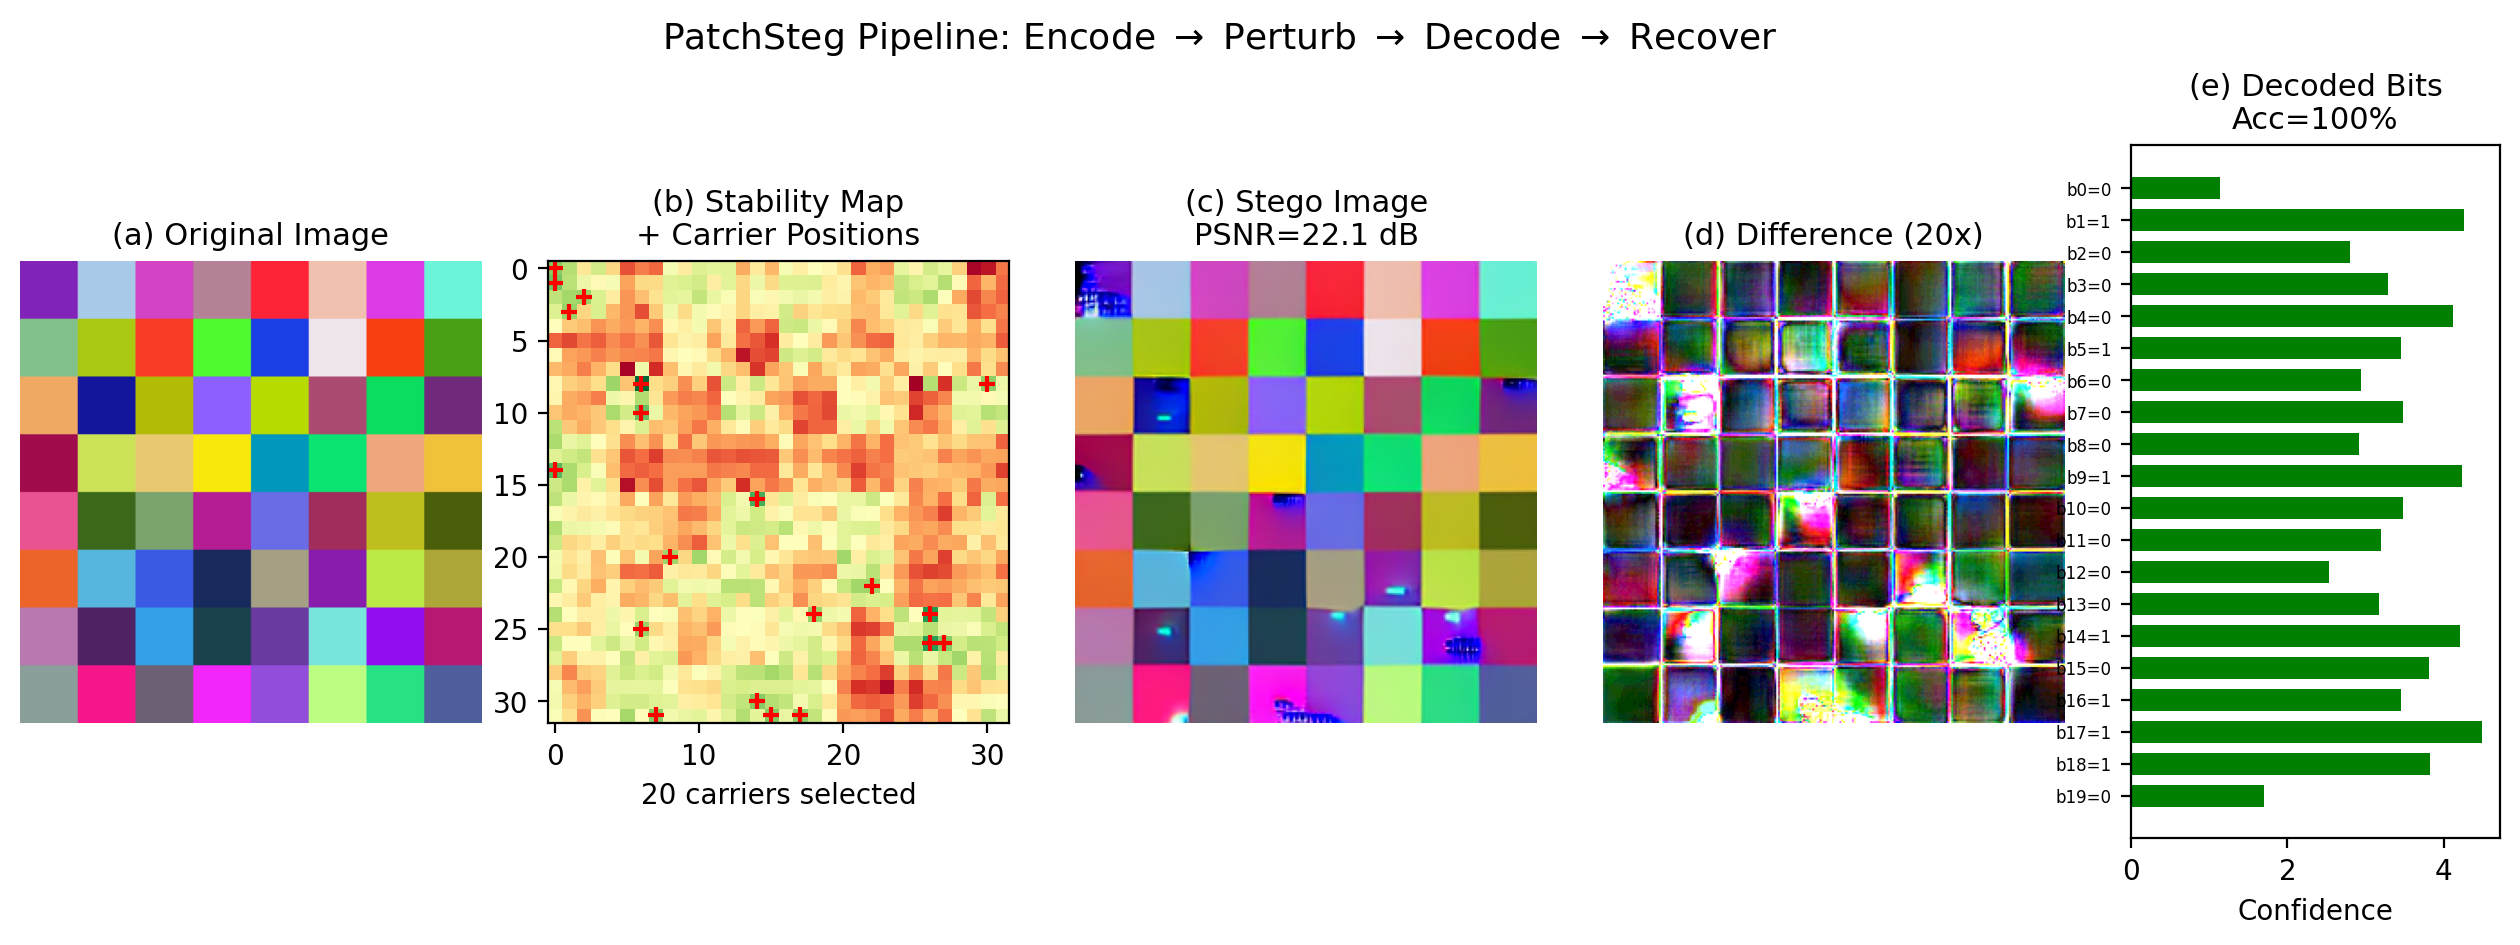
\includegraphics[width=0.92\textwidth]{../figures/hero_pipeline.png}
\caption{PatchSteg in an agentic image-sharing pipeline. The sender writes signed perturbations into VAE latent carriers, posts the decoded image, and the receiver recovers the message by re-encoding. A monitor that sees only pixels and captions may miss the representation-level channel.}
\label{fig:pipeline}
\end{figure*}

\section{Threat Model}

\textbf{Sender.}
The sender can access a cover image, encode it with a compatible VAE, apply small latent perturbations, and share the decoded image through an agent workspace or tool output.

\textbf{Receiver.}
The receiver can access the shared image, re-encode it with a compatible VAE, and derive the same carrier positions and perturbation direction from a shared seed. The baseline protocol assumes the receiver can reproduce a clean cover latent or clean round-trip baseline. Blind variants are exploratory and not required for the main claim.

\textbf{Monitor.}
The monitor may inspect pixels, captions, metadata, and optionally run statistical detectors or sanitizers. We distinguish pixel-only monitors from representation-aware monitors because PatchSteg targets the gap between visible content and model-readable latent state.

\textbf{Out of scope.}
We do not claim a complete deployment attack against arbitrary VLMs, nor a fully adaptive attack against a learning monitor. The purpose is to establish and diagnose a plausible communication channel in shared image infrastructure.

\section{Related Work}

\textbf{Secret collusion among agents.}
Motwani et al. demonstrate hidden text channels between language agents \citep{motwani2024secret}. PatchSteg studies the multimodal analogue: agents can coordinate through images whose visible content appears benign.

\textbf{Latent image steganography and watermarking.}
RoSteALS trains latent steganographic models \citep{bui2023rosteals}. Stable Signature \citep{fernandez2023stable}, Tree-Ring Watermarking \citep{wen2023treering}, and Gaussian Shading \citep{yang2024gaussian} focus on watermarking or generation-time mechanisms. PSyDUCK studies training-free latent-diffusion steganography using trajectory control \citep{jiang2025psyduck}. PatchSteg is post-hoc: it modifies existing-image VAE latents with no training.

\textbf{Representation-level monitoring.}
Prior work on VAE geometry shows that latent spaces have structured directions \citep{rolinek2019variational}. For agent security, this means visible outputs may not exhaust the information available to model-aware receivers.

\section{PatchSteg}

\subsection{Channel Construction}

Let $z\in\mathbb{R}^{4\times H/8\times H/8}$ be the VAE latent of a cover image. Sender and receiver derive a unit direction $d\in\mathbb{R}^4$ and carrier set $\mathcal{C}=\{(r_i,c_i)\}_{i=1}^K$ from a shared seed. To encode bit $b_i$:
\begin{equation}
z_{:,r_i,c_i}^{\,\mathrm{stego}}=z_{:,r_i,c_i}+(2b_i-1)\epsilon d .
\end{equation}
The sender decodes $z^{\mathrm{stego}}$ and shares the image.

The receiver re-encodes the image to $z'$ and compares it with a clean round-trip baseline $\bar z=\mathrm{Enc}(\mathrm{Dec}(z))$:
\begin{equation}
\hat b_i=\mathbb{1}\left[\langle z'_{:,r_i,c_i}-\bar z_{:,r_i,c_i},d\rangle>0\right].
\end{equation}

\subsection{Carrier Stability}

Carrier positions differ substantially in how well they preserve signed perturbations. We define:
\begin{equation}
S_{r,c}(x;d,\epsilon)=
\left\langle
\mathrm{Enc}(\mathrm{Dec}(z+\epsilon d_{r,c}))_{:,r,c}-\bar z_{:,r,c},d
\right\rangle .
\end{equation}
Ranking carriers by $S$ gives a reproducible diagnostic and improves reliability at lower perturbation strengths.

\begin{table}[t]
\caption{Round-trip validation with random carriers at $256\times256$.}
\label{tab:roundtrip}
\centering
\begin{small}
\begin{tabular}{cccc}
\toprule
$\epsilon$ & Carriers & Bit Acc. (\%) & PSNR (dB) \\
\midrule
0.5 & 5  & 80.0  & 32.0 \\
0.5 & 20 & 52.5  & 32.0 \\
2.0 & 5  & 90.0  & 31.8 \\
2.0 & 20 & 75.0  & 31.7 \\
5.0 & 5  & 100.0 & 31.4 \\
5.0 & 20 & 100.0 & 30.7 \\
\bottomrule
\end{tabular}
\end{small}
\end{table}

\section{Evaluation}

\subsection{Spatial And Content Dependence}

Stability is spatially non-uniform: averaged scores at $\epsilon=5.0$ range from 0.98 to 3.48 across positions. Stability-selected carriers at $\epsilon=2.0$ achieve 100\% bit accuracy with 20 carriers on a structured color-block image, compared with 75\% for random carriers in the initial validation.

\begin{figure}[t]
\centering
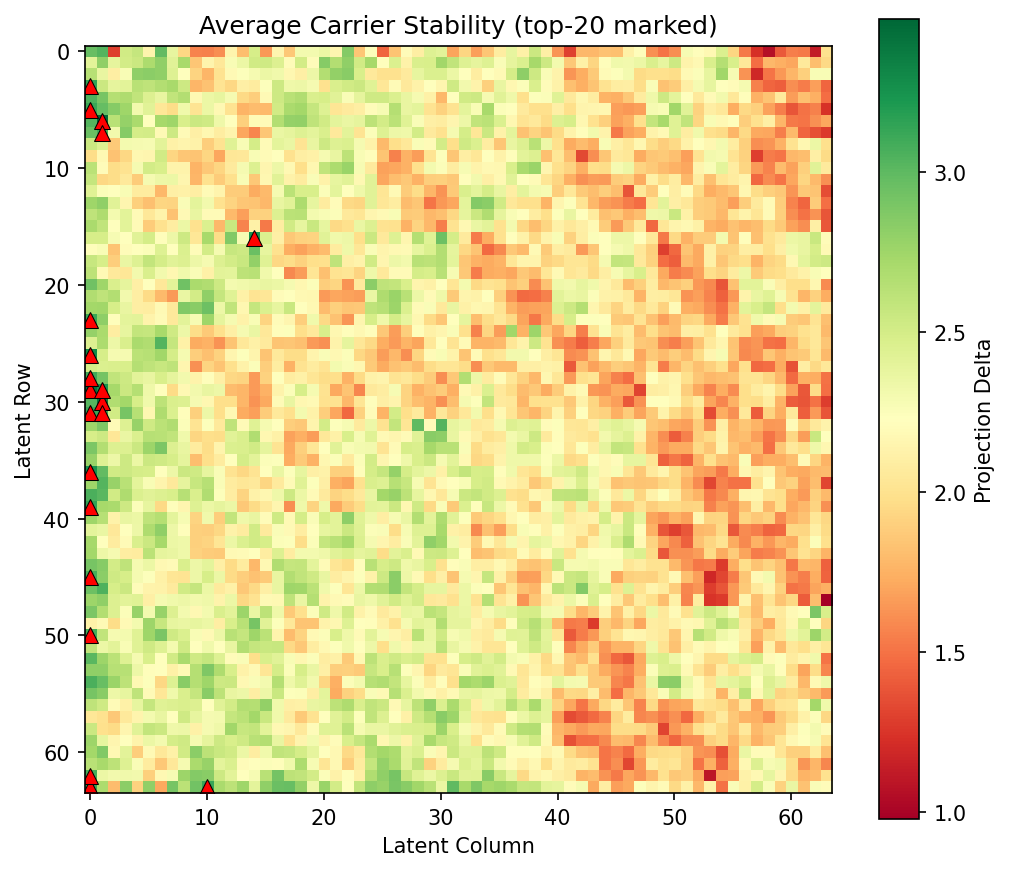
\includegraphics[width=0.78\columnwidth]{../figures/carrier_stability_avg.png}
\caption{Carrier-stability map. The channel exists because some spatial latent positions preserve signed perturbations much better than others.}
\label{fig:stability}
\end{figure}

Content matters. Smooth gradients are poor carriers, while textured images are reliable. Across 50 synthetic images, entropy and high-frequency energy correlate with bit accuracy (Pearson $r=0.555$ and $0.534$).

\begin{figure}[t]
\centering
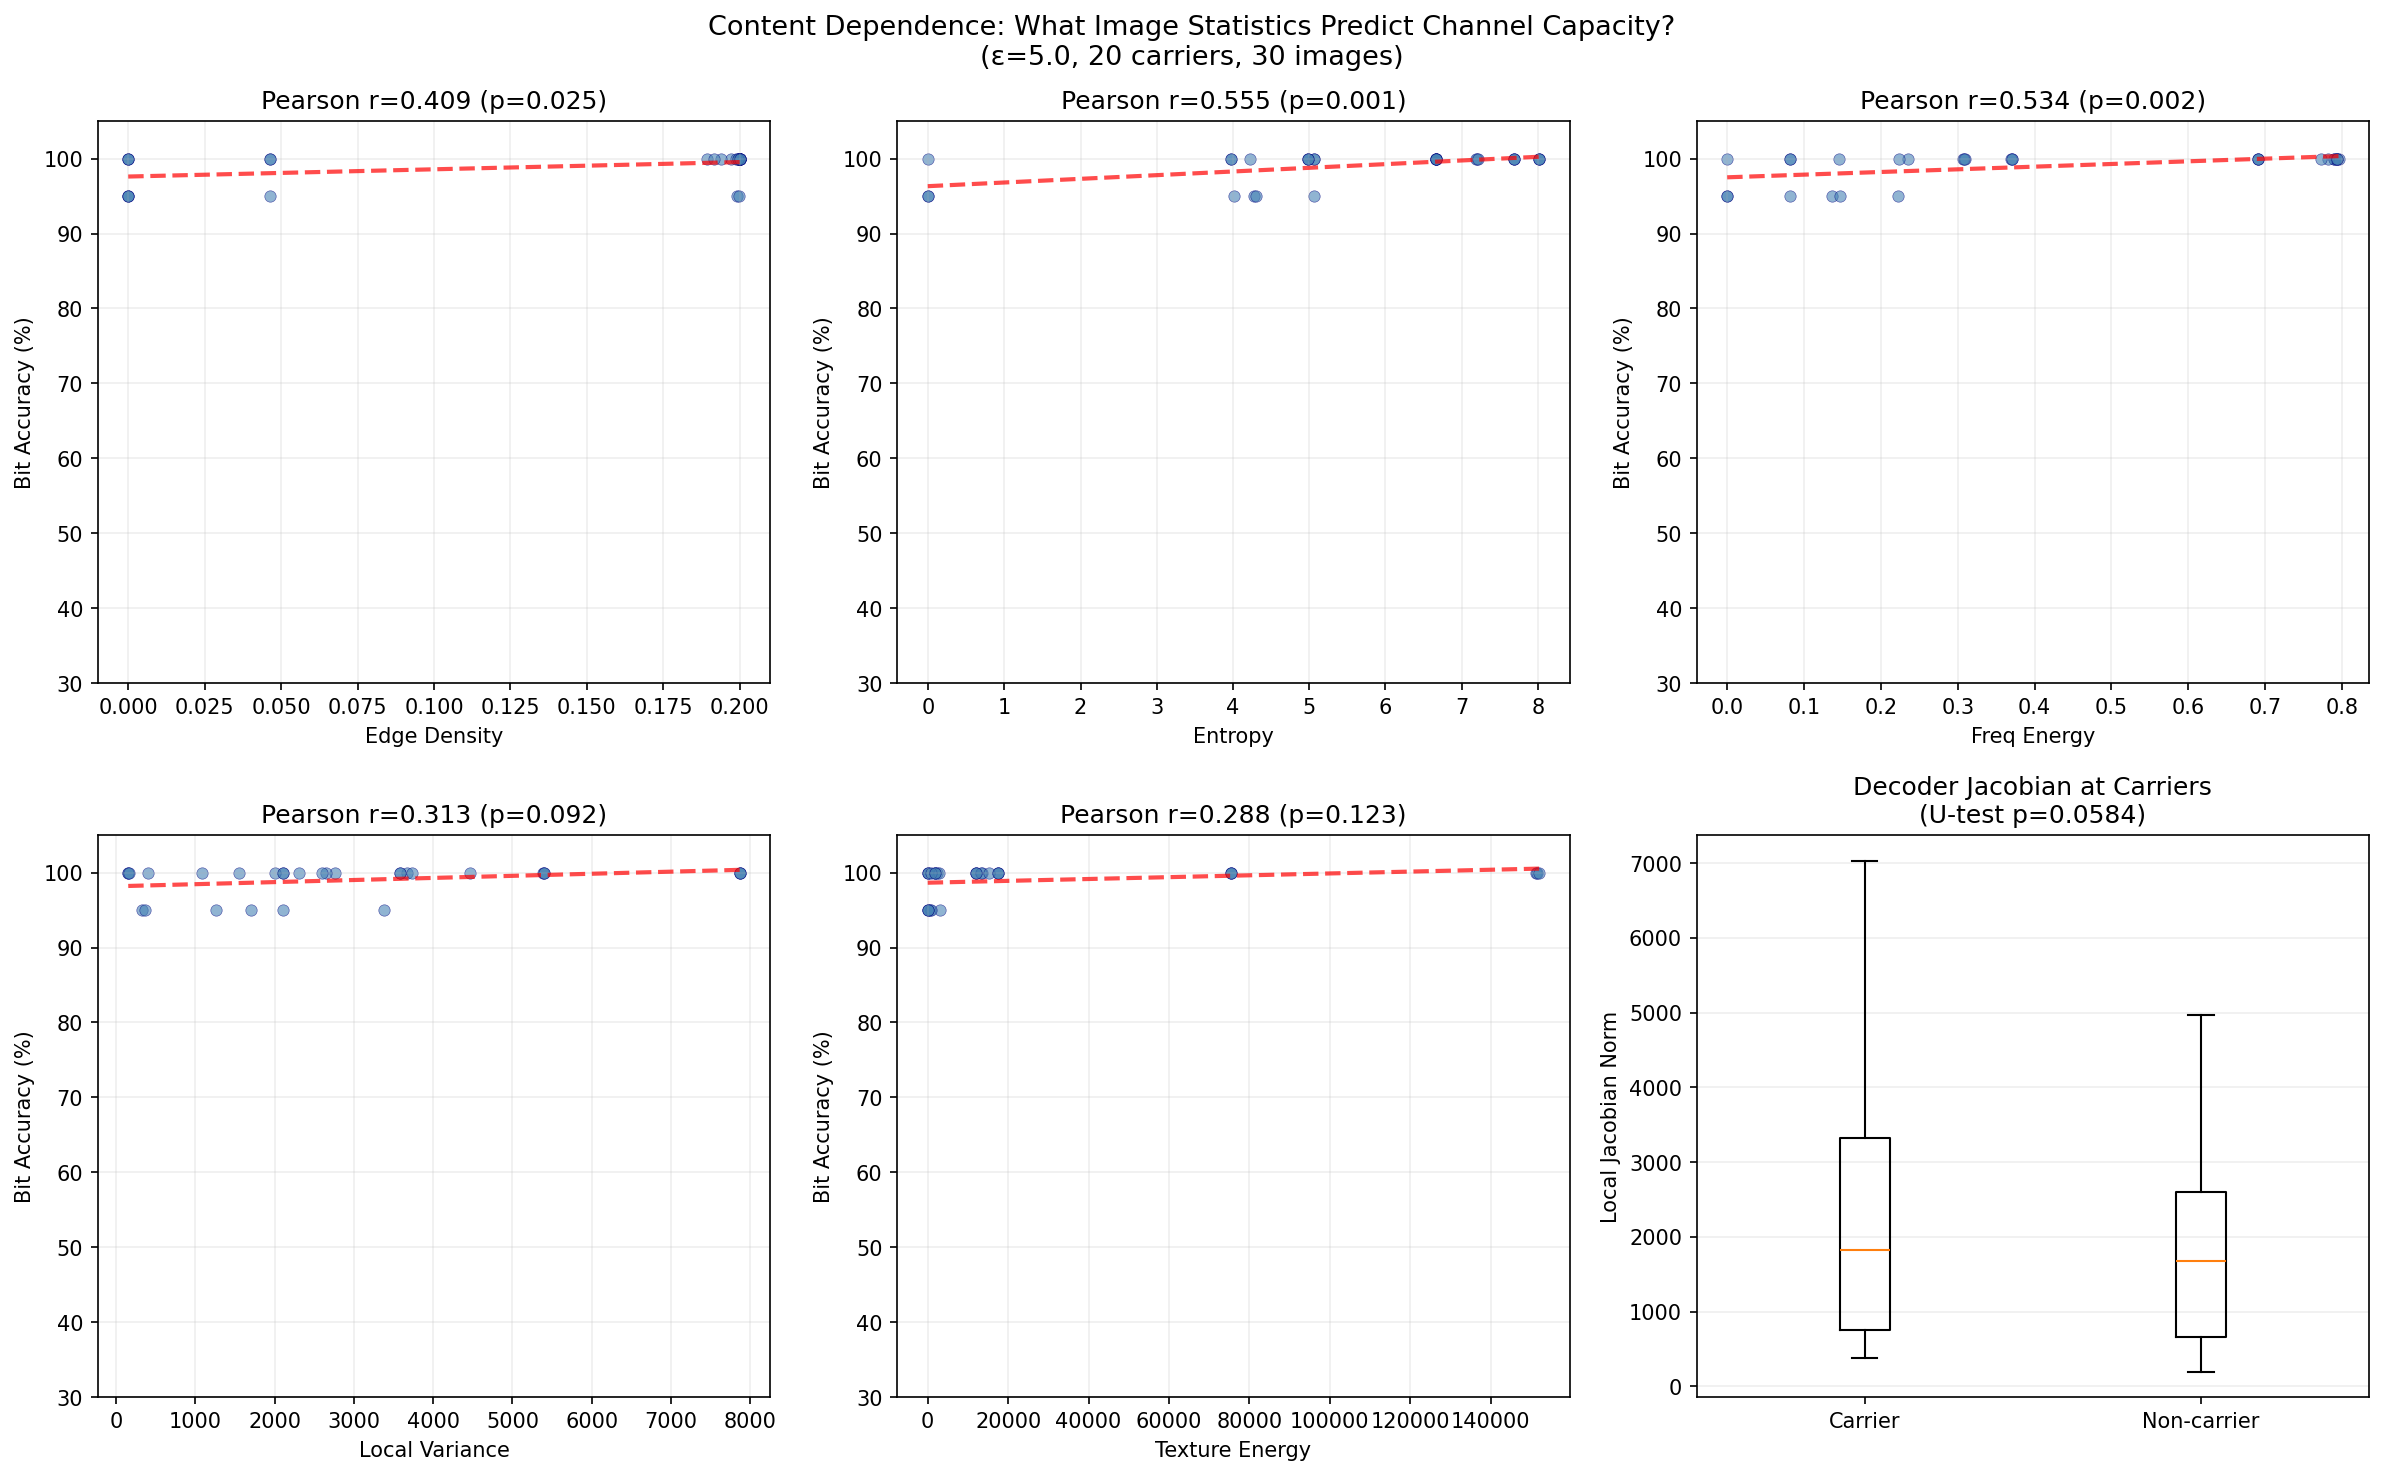
\includegraphics[width=\columnwidth]{../figures/content_science.png}
\caption{Content dependence. Image statistics and local geometry predict when the channel is reliable.}
\label{fig:content}
\end{figure}

\subsection{Natural Images And Model Generality}

On 300 CIFAR-10 images resized to $256\times256$, PatchSteg reaches 98.2\% bit accuracy at $\epsilon=2.0$ with 95\% CI [97.8, 98.7], and 98.5\% at $\epsilon=5.0$ with 95\% CI [98.0, 98.9]. Mean PSNR values are 38.6 dB and 28.9 dB. These results are strong enough to establish the channel but should be supplemented with native high-resolution images.

\begin{figure}[t]
\centering
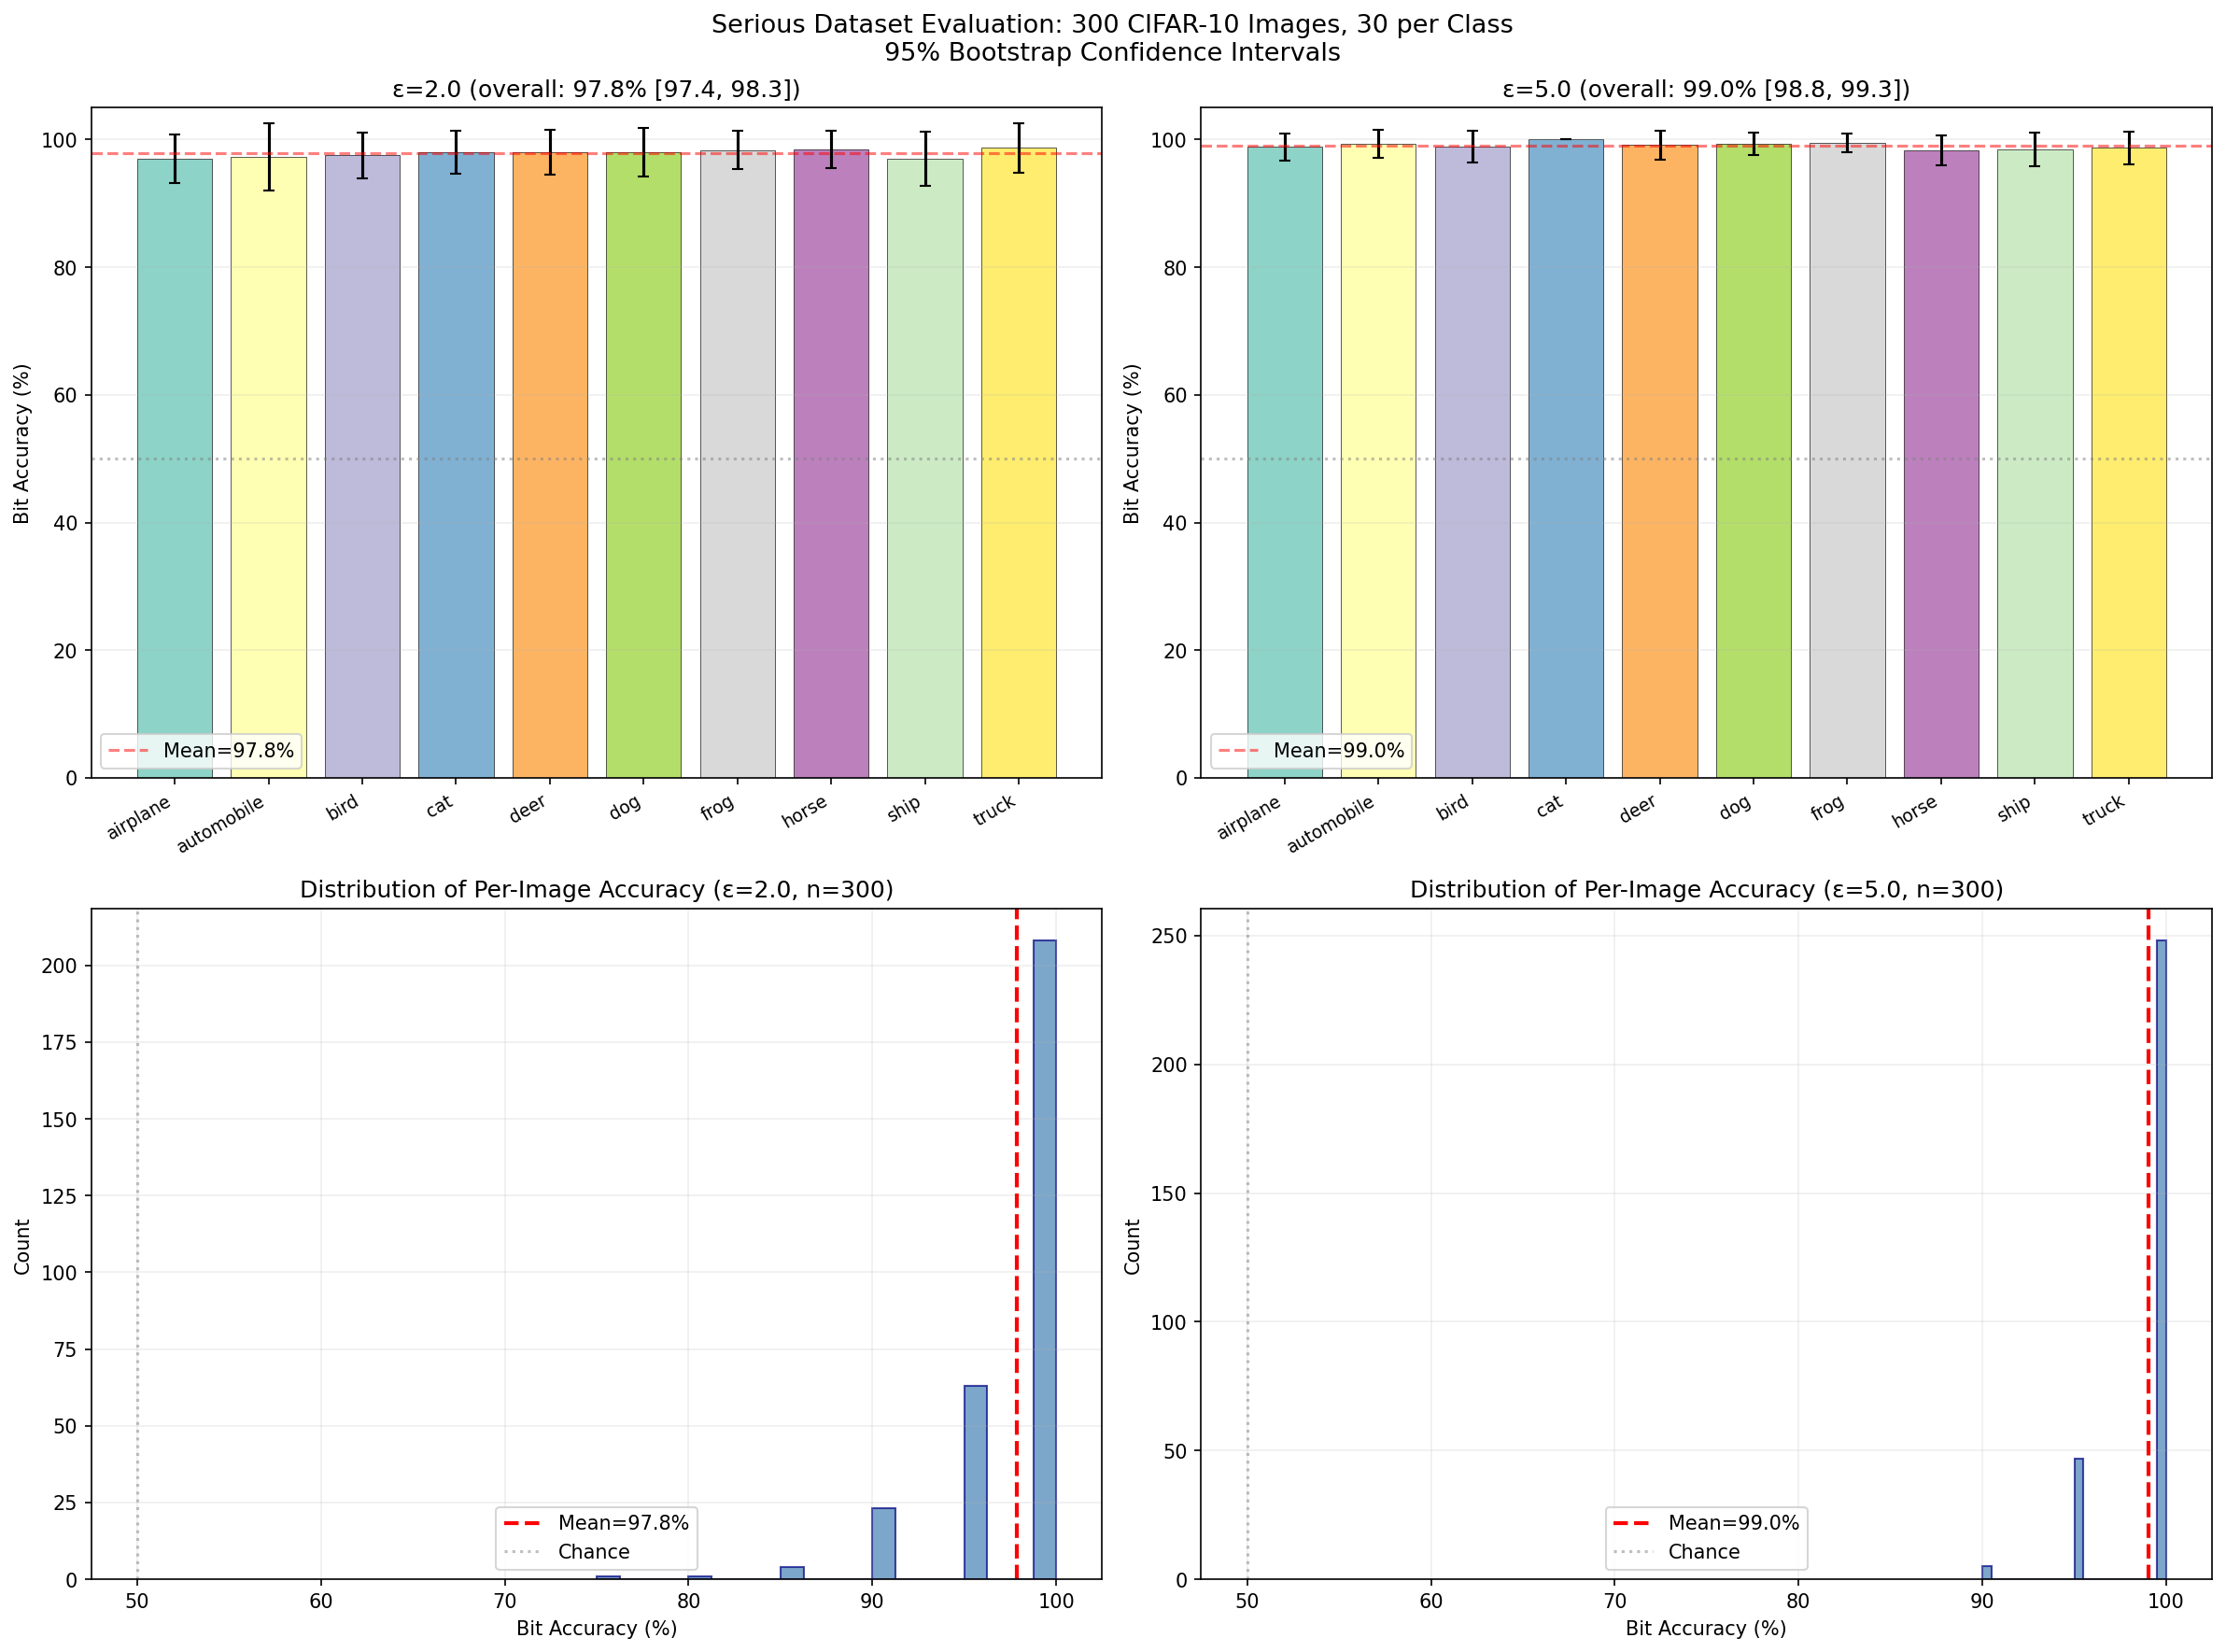
\includegraphics[width=\columnwidth]{../figures/serious_dataset.png}
\caption{Natural-image evaluation. Recovery is high across CIFAR-10 classes, with variation consistent with content dependence.}
\label{fig:natural}
\end{figure}

The channel generalizes across SD-VAE-MSE, SD-VAE-EMA, and SDXL-VAE, and related checkpoints support cross-model decoding.

\begin{figure}[t]
\centering
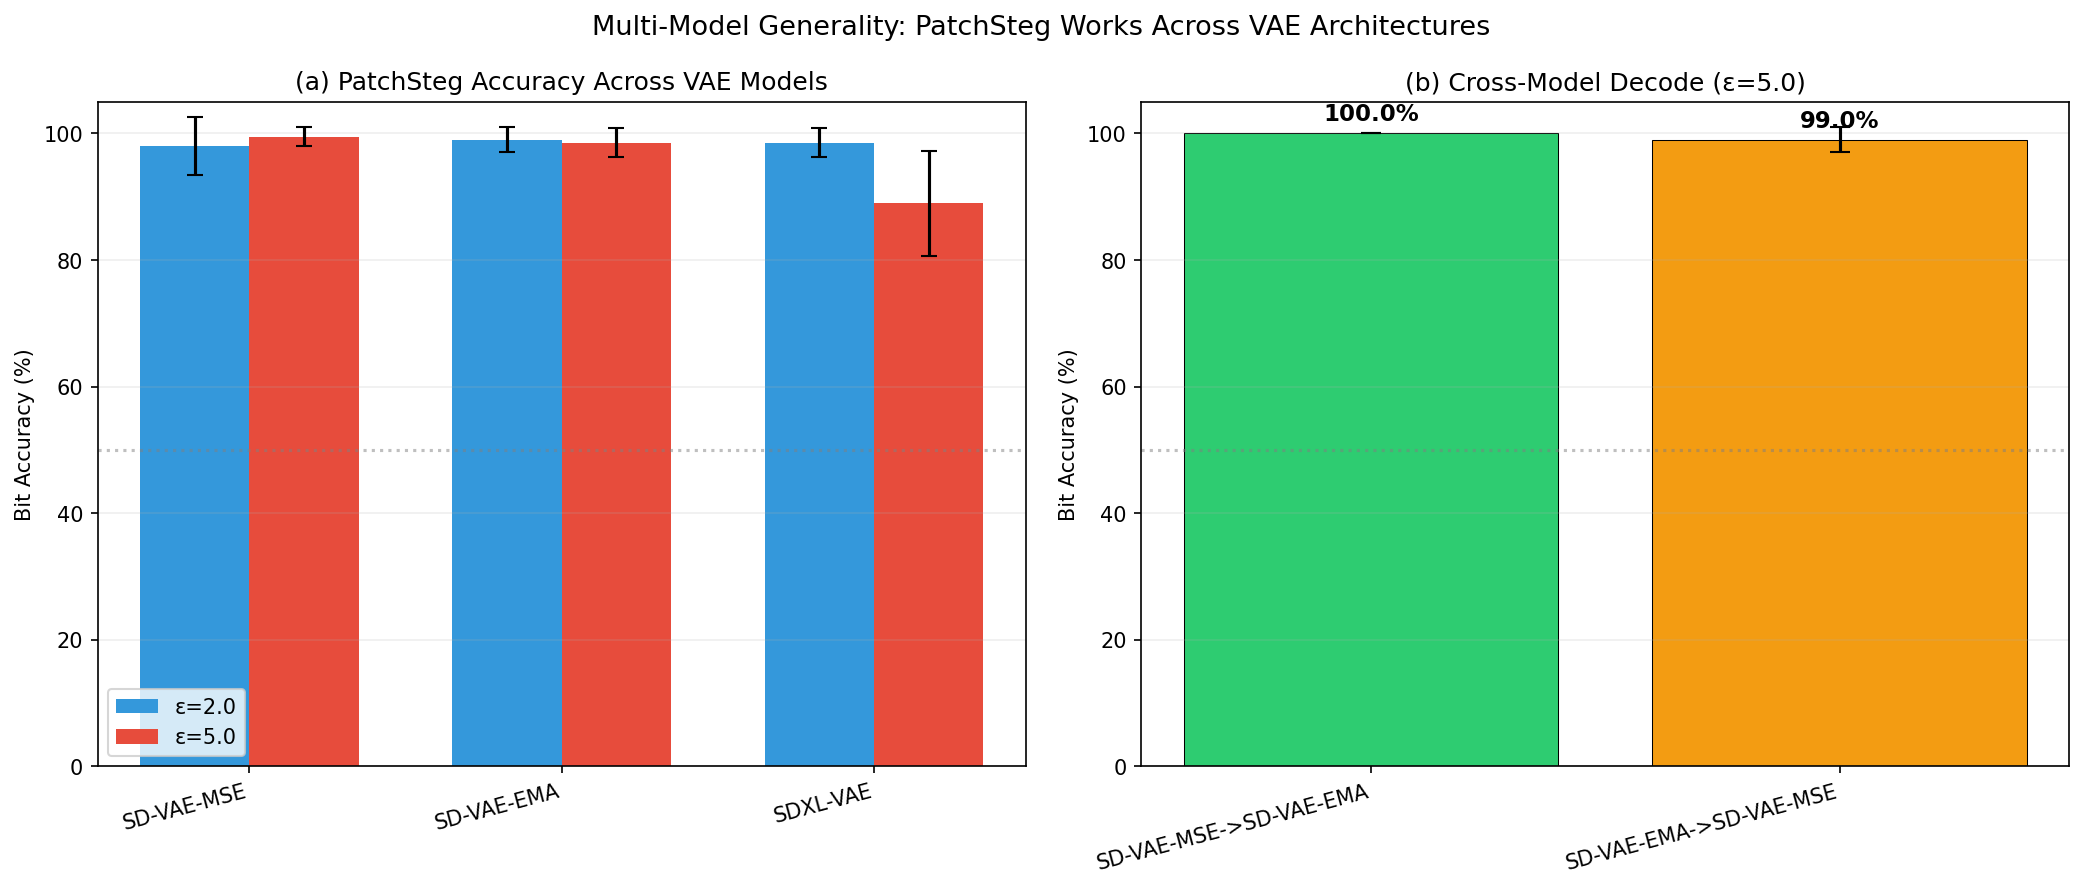
\includegraphics[width=\columnwidth]{../figures/multimodel.png}
\caption{Multi-model evaluation. Compatibility between related VAE checkpoints is an important security consideration for agent platforms.}
\label{fig:multimodel}
\end{figure}

\subsection{Monitoring And Robustness}

A latent-statistics logistic regression detector yields AUC 0.44 at $\epsilon=1.0$, 0.68 at $\epsilon=2.0$, 0.93 at $\epsilon=5.0$, and 0.97 at $\epsilon=10.0$. Stronger pixel-residual and spectral detectors perform better in some protocols. Thus, the right security conclusion is not that PatchSteg is undetectable, but that monitoring assumptions matter.

\begin{figure}[t]
\centering
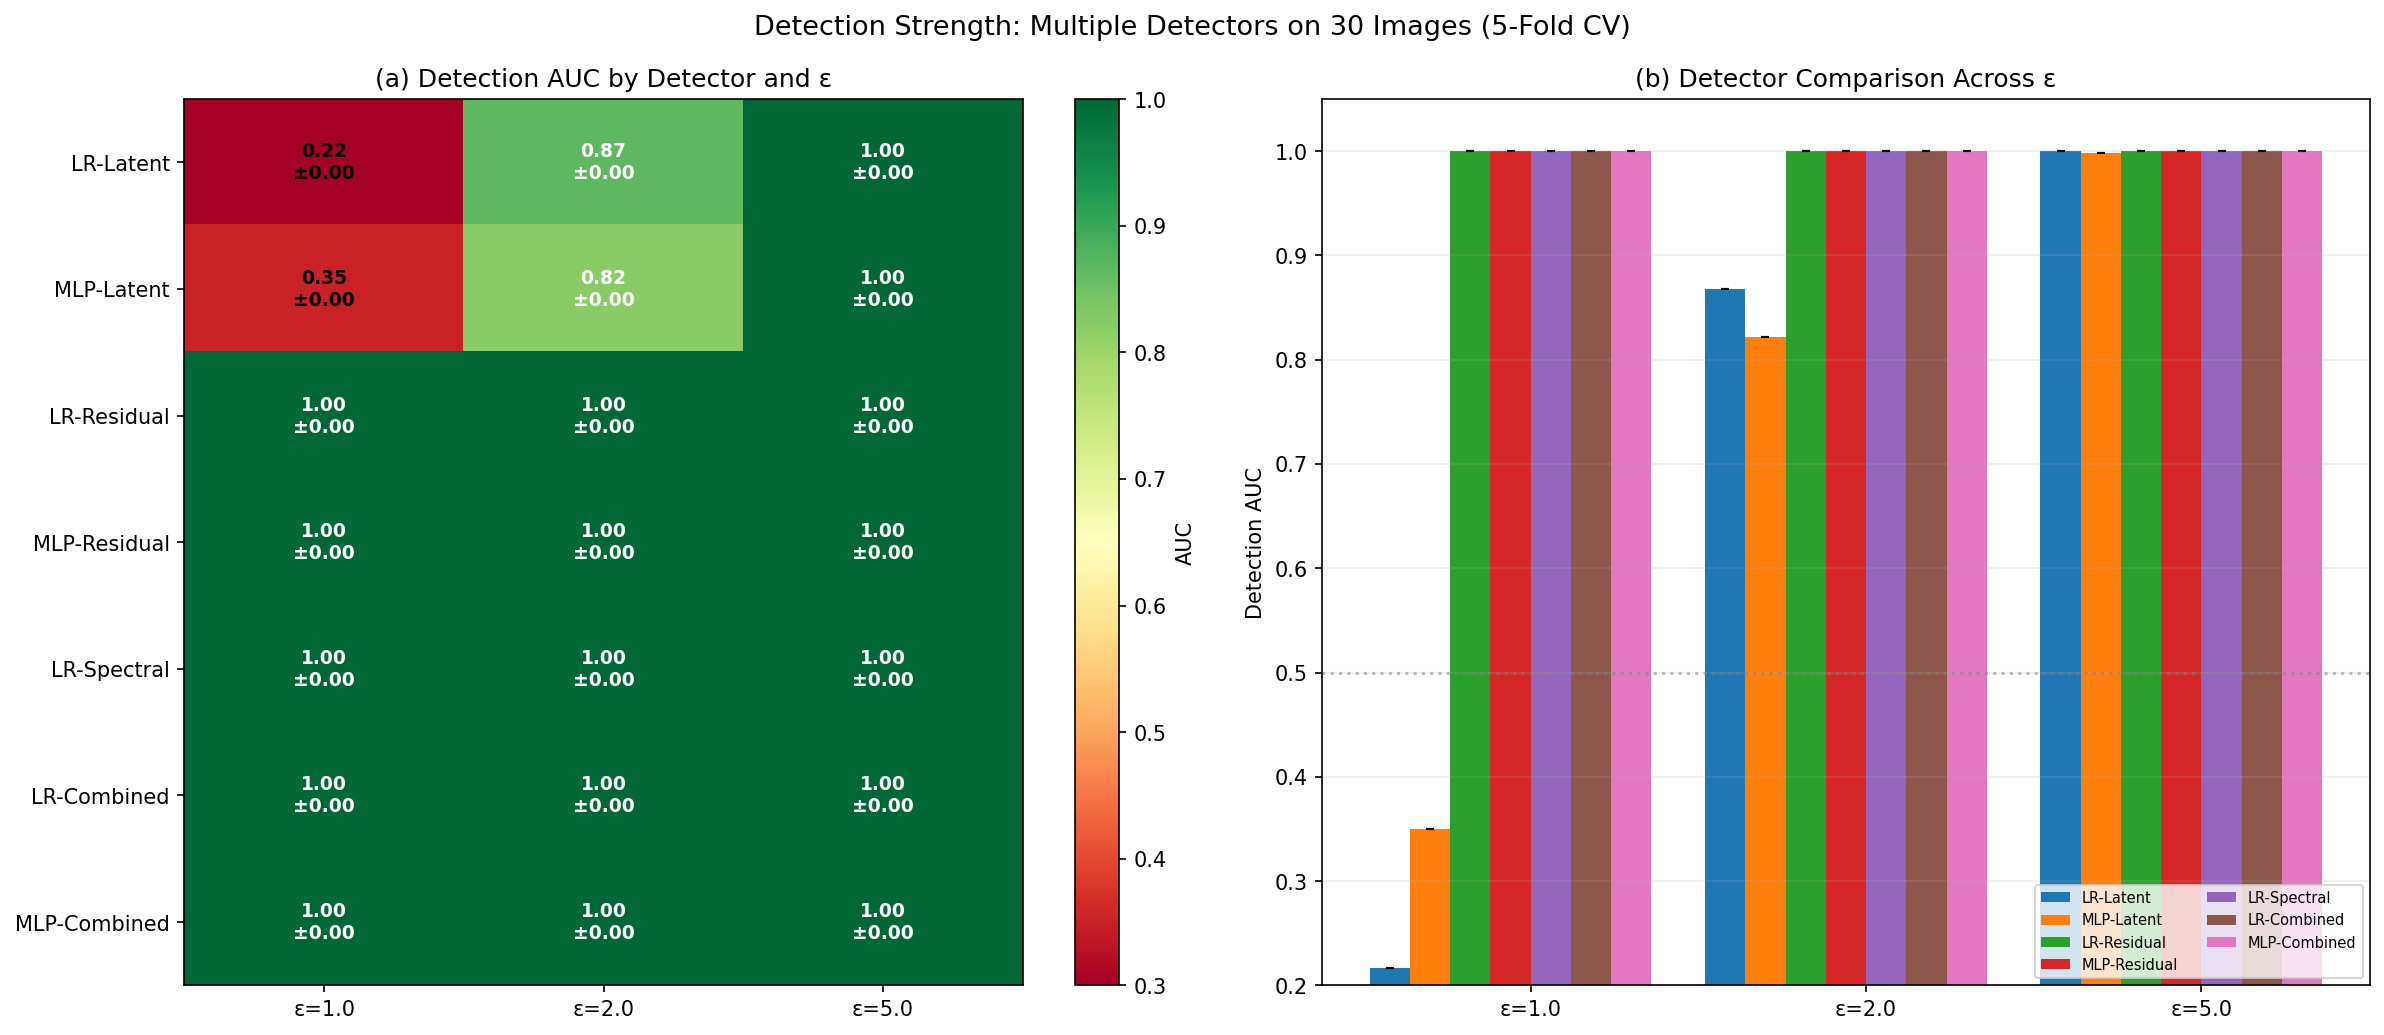
\includegraphics[width=\columnwidth]{../figures/detection_strength.png}
\caption{Detector sweep. Representation-aware and pixel-residual detectors reveal a monitoring arms race rather than a simple yes/no defense.}
\label{fig:detection}
\end{figure}

The channel can survive distortions that preserve spatial carrier alignment. In deployment-style tests, $\epsilon=5.0$ survives VAE re-encoding (99\%), screenshot simulation (98.5\%), JPEG Q=10 (96.5\%), resize to 25\% (92\%), and additive noise with $\sigma=0.10$ (98\%). Cropping is more destructive because it changes carrier alignment.

\section{Implications For Multi-Agent Systems}

PatchSteg changes the monitoring question from "does the image look suspicious?" to "what information can another model recover from this image?" For agent platforms, this suggests three defensive directions. First, monitors should specify whether they are pixel-only or representation-aware. Second, shared image infrastructure may need latent sanitization, not only caption review. Third, evaluations should include adaptive senders and operating-point detector metrics, such as precision and recall at fixed low false-positive rates.

The most important missing experiment is an end-to-end agentic scenario: sender and receiver agents exchanging images through a shared workspace while a third monitor inspects pixels and captions. We treat this as immediate future work rather than claiming deployment realism from the VAE-level channel alone.

\section{Limitations}

The baseline protocol requires a compatible VAE, shared seed, and shared cover or clean round-trip baseline. The main natural-image evaluation uses upscaled CIFAR-10; native high-resolution images should be added. PSNR should be supplemented with SSIM and LPIPS. Current sanitizer and adaptive-sender experiments are preliminary. Finally, this paper establishes a channel and diagnostics, not a complete attack on arbitrary multimodal agents.

\section{Conclusion}

PatchSteg demonstrates that shared images can carry model-readable latent information between multimodal agents. The result is technically simple but security-relevant: pixel-level monitoring does not necessarily capture the information available to another model in the pipeline. Agent security evaluations should therefore include representation-level channels, detector operating points, and sanitization tradeoffs.

\bibliography{../main}
\bibliographystyle{../../icml2026/icml2026}

\clearpage
\appendix

\section{Appendix Index}

\begin{table*}[t]
\caption{Supplementary figures retained from the longer internal draft. They provide monitoring and robustness context but are not required for the main AIWILD claim.}
\label{tab:appendix_index}
\centering
\begin{small}
\begin{tabular}{lll}
\toprule
Appendix & Artifact & Purpose \\
\midrule
\ref{app:monitoring} & Deployment robustness & Shows distortion sensitivity in image-sharing pipelines. \\
\ref{app:monitoring} & Detector ROC curves & Provides detailed detector behavior. \\
\ref{app:monitoring} & Cross-method transfer & Shows pilot transfer between detector/attack variants. \\
\ref{app:variants} & CDF detectability & Documents exploratory blind-decoding variant. \\
\ref{app:variants} & Quantile sanitizer & Documents exploratory disruption/fidelity tradeoff. \\
\bottomrule
\end{tabular}
\end{small}
\end{table*}

\clearpage
\section{Additional Robustness And Monitoring Figures}
\label{app:monitoring}

\begin{figure*}[t]
\centering
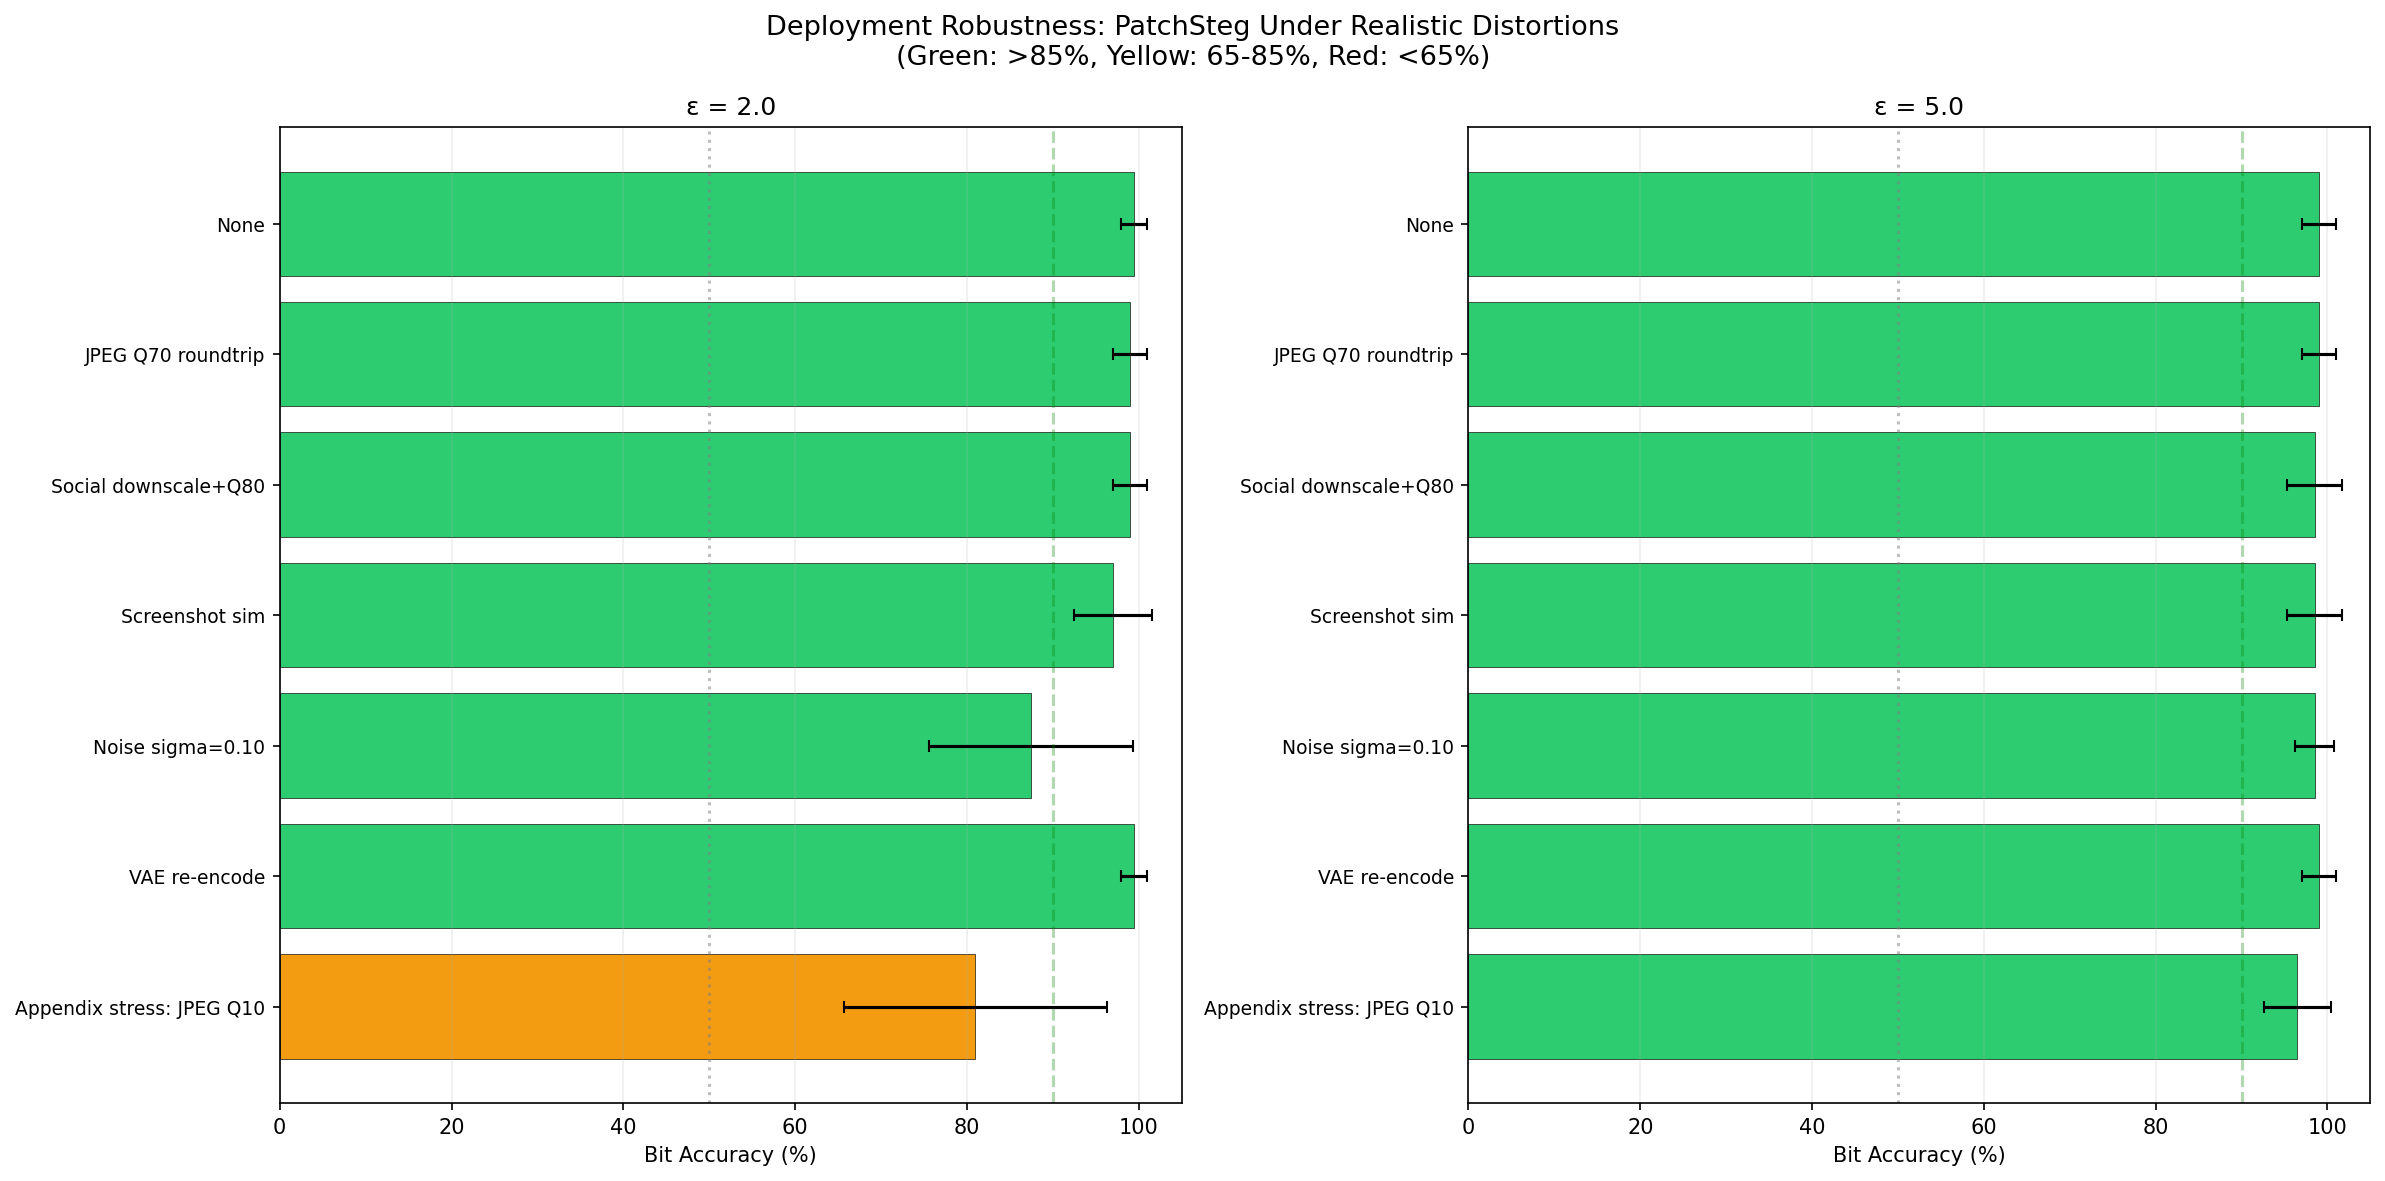
\includegraphics[width=0.82\textwidth]{../figures/deployment_robustness.png}
\caption{Deployment robustness across image transformations.}
\end{figure*}

\begin{figure*}[t]
\centering
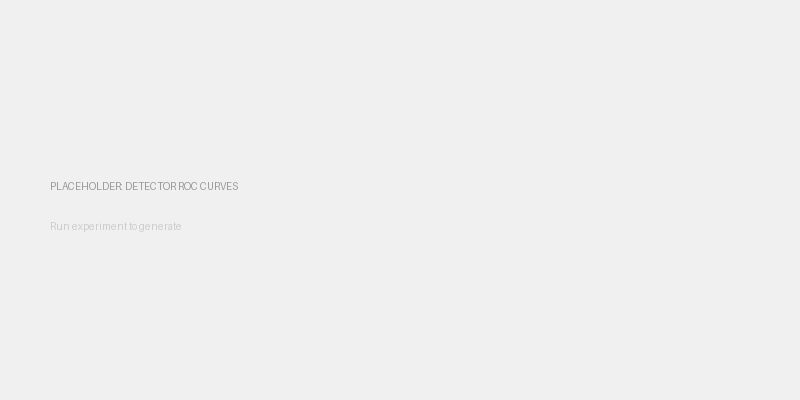
\includegraphics[width=0.82\textwidth]{../figures/detector_roc_curves.png}
\caption{ROC curves for a stronger latent steganalysis detector.}
\end{figure*}

\begin{figure*}[t]
\centering
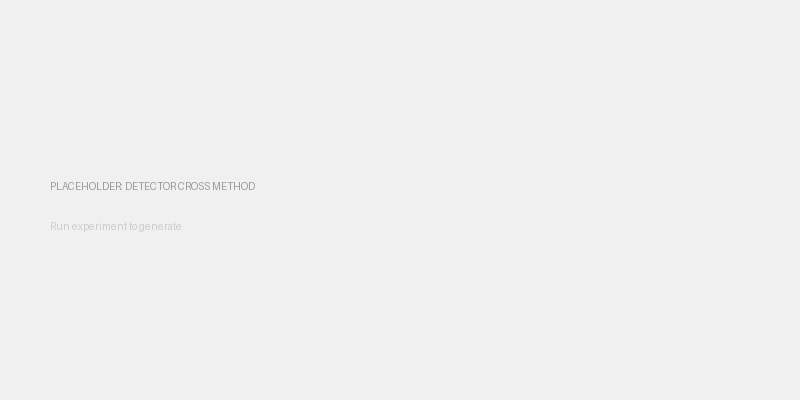
\includegraphics[width=0.72\textwidth]{../figures/detector_cross_method.png}
\caption{Cross-method detector transfer pilot.}
\end{figure*}

\clearpage
\section{Exploratory Variants And Defenses}
\label{app:variants}

\begin{figure*}[t]
\centering
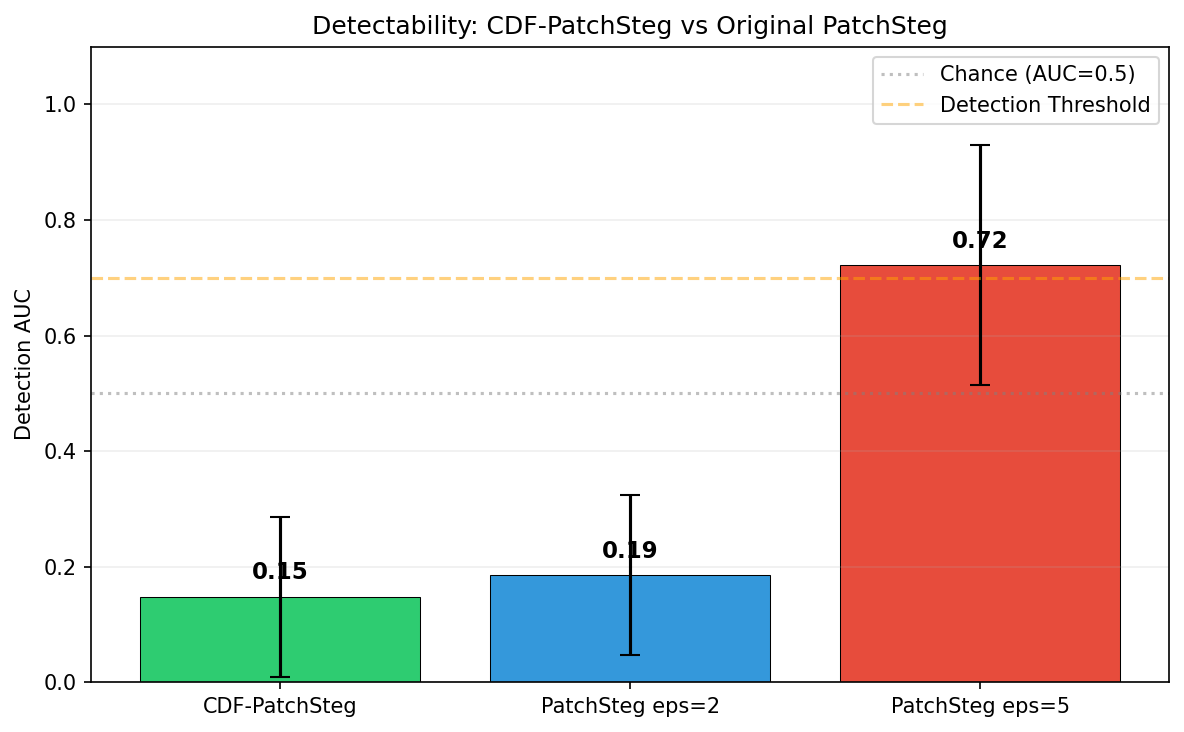
\includegraphics[width=0.72\textwidth]{../figures/cdf_detectability.png}
\caption{CDF-PatchSteg pilot detectability. This is exploratory and not central to the main AIWILD claim.}
\end{figure*}

\begin{figure*}[t]
\centering
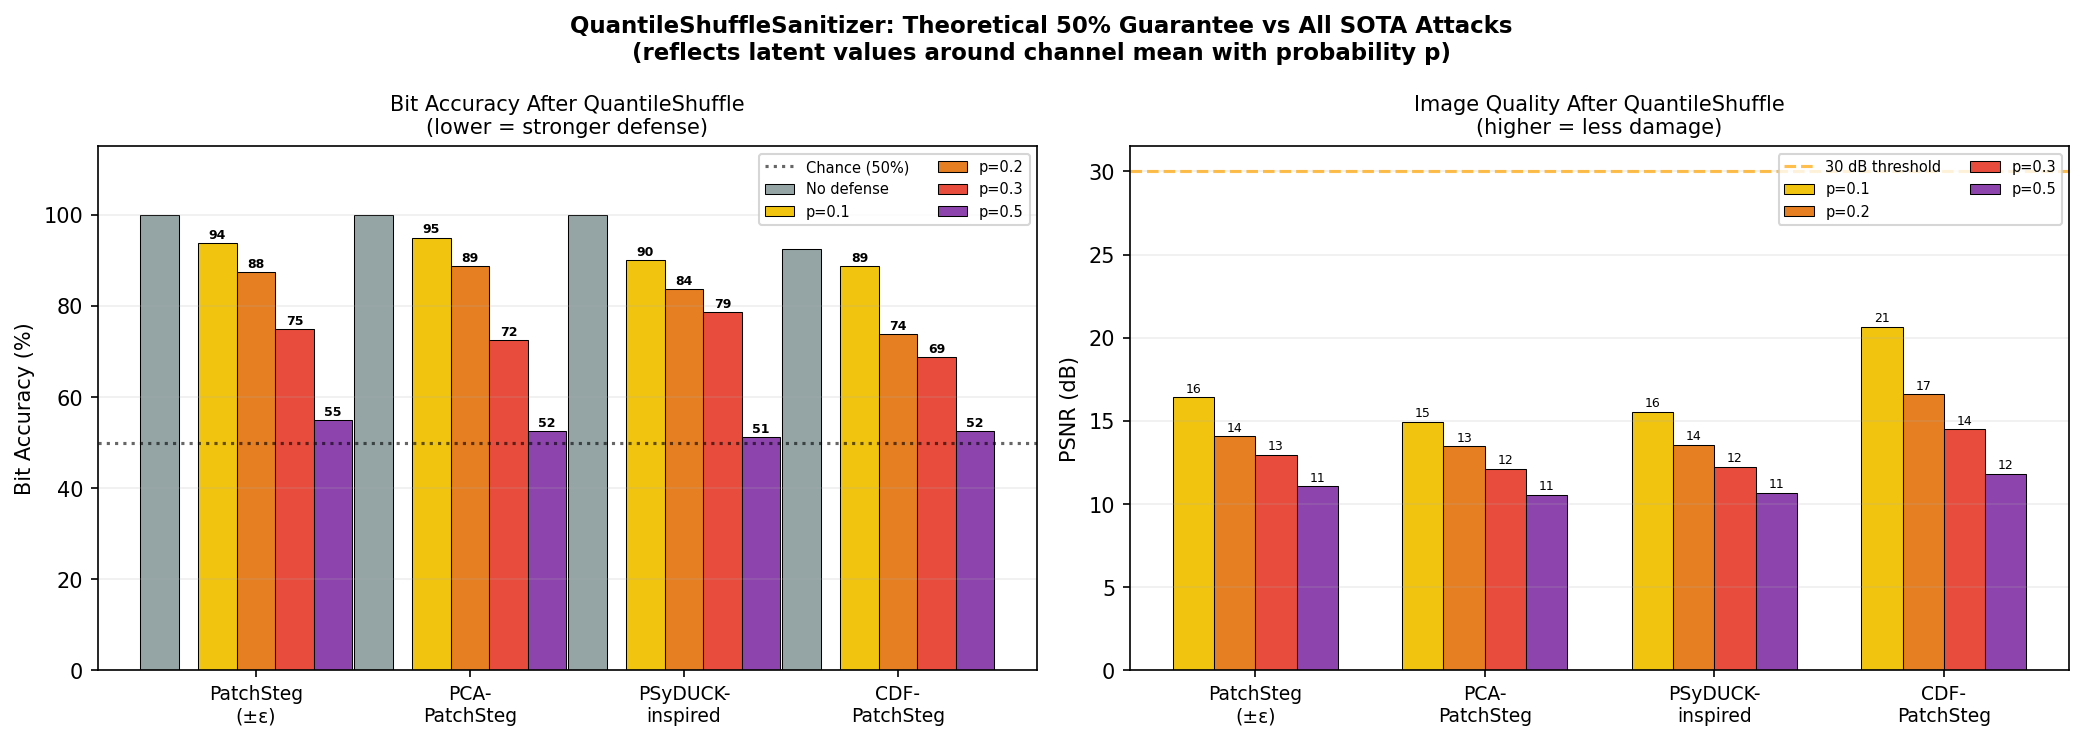
\includegraphics[width=0.82\textwidth]{../figures/quantile_sanitizer_results.png}
\caption{Quantile-sanitizer pilot. Strong disruption requires substantial latent modification.}
\end{figure*}

\end{document}
